%!TEX TS-program = xelatex
\documentclass[]{friggeri-cv}
\usepackage[brazil,english]{babel}
\usepackage{xltxtra}
\defaultfontfeatures{Ligatures=TeX}
\usepackage{afterpage}
\usepackage{hyperref}
\usepackage{hyphenat}
\usepackage{color}
\usepackage{xcolor}
\usepackage{fancyhdr}
\usepackage{multilanguage}

\setdoclang{br}{brazil}
%\setdoclang{en}{english}

\hypersetup{
    colorlinks,
    linkcolor={red!50!black},
    citecolor={blue!50!black},
    urlcolor={blue!80!black},
    pdfborder={0 0 0},
}

\pagestyle{fancy}
\lhead{}
\chead{}
\rhead{}
\rfoot{{%
    \footnotesize{%
        \langif{br}{%
        %lang pt-br
            Veja a última versão deste documento em:
            \href{https://github.com/diraol/cv/releases/}{https://github.com/diraol/cv/releases/}%
        }{%
        %lang en
            See the lastest version of this document at:
            \href{https://github.com/diraol/cv/releases/}{https://github.com/diraol/cv/releases/}%
        }
}}}
\renewcommand{\headrulewidth}{0pt}
\renewcommand{\footrulewidth}{0pt}

\hypersetup{
    pdftitle={Diego Rabatone Oliveira Resume},
    pdfauthor={Diego Rabatone Oliveira},
    pdfsubject={Resume/CV},
    pdfkeywords={Diego Rabatone, diraol, cv, resume},
    colorlinks=false,       % no lik border color
   allbordercolors=white    % white border color for all
}
%\addbibresource{bibliography.bib}
\RequirePackage{xcolor}
\definecolor{pblue}{HTML}{0395DE}

\begin{document}
\thispagestyle{empty}
\pagenumbering{gobble}% Remove page numbers (and reset to 1)
%%%%%%%%%%%%%%%%%%%%%%%%%%%%%%%%%%%%%%%%%%
%\langif{br}{%
%% text for lang pt-br
%
%}{%
%% text for lang pt-br
%
%}
%\langif{br}{}{}
%%%%%%%%%%%%%%%%%%%%%%%%%%%%%%%%%%%%%%%%%%
\header{Diego}{Rabatone O.}{\langif{br}{Engenheiro de Computação}{Computer Engineer}}

% Fake text to add separator
\fcolorbox{white}{gray}{\parbox{\dimexpr\textwidth-2\fboxsep-2\fboxrule}{%

}}

% In the aside, each new line forces a line break
\begin{aside}
  \section{\langif{br}{Endereço}{Address}}
    São Paulo, SP, \langif{br}{Brasil}{Brazil}
    ~
  \section{\langif{br}{Telefone}{Tel}}
    +55 11 9-8231-4249
    ~
  \section{\langif{br}{e-mail}{Mail}}
    \href{mailto:diraol@diraol.eng.br}{\textbf{diraol@}\\diraol.eng.br}
    \href{mailto:diraol@members.fsf.org}{\textbf{diraol@}\\members.fsf.org}
    \href{mailto:diraol@usp.br}{\textbf{diraol@}\\usp.br}
    ~
  \section{IRC}
    \#diraol (at) irc.freenode.net
    ~
  \section{Twitter}
    \href{http://twitter.com/diraol}{@diraol}
    ~
  \section{LinkedIn}
    \href{http://br.linkedin.com/in/diraol}{br.linkedin.com/in/diraol}
    ~
  \section{Web \& Git}
    \href{http://cv.diraol.eng.br}{cv.diraol.eng.br}
    \href{https://github.com/diraol}{github.com/diraol}
    ~
  \section{\langif{br}{Idiomas}{Languages}}
    \textbf{\langif{br}{Português}{Portuguese}}
\includegraphics[scale=0.40]{img/5stars.png}
    \textbf{\langif{br}{Inglês}{English}}
\includegraphics[scale=0.40]{img/5stars.png}
    \textbf{\langif{br}{Francês}{French}}
\includegraphics[scale=0.40]{img/1stars.png}
    \textbf{\langif{br}{Espanhol}{Spanish}}
\includegraphics[scale=0.40]{img/1stars.png}
\end{aside}

\sectionlang{br}{Experiência}
\sectionlang{en}{Experience}
\begin{entrylist}
  \entry
    {\langif{br}{Out/09 - Hoje}{Oct/09 - now}}
    {\langif{br}{Co-fundador, coordenador e membro}{Co-Founder, coordinator and member}}
    {\href{http://polignu.org}{PoliGNU}}
    {\langif{br}{PoliGNU - Grupo de Estudos de Software Livre da Poli-USP}{PoliGNU - Poli-USP Free Software Studies Group}\\
    \langif{br}{Organização e planejamento de atividades e grupos de discussão}{Organization and planning of activities and discussion groups}\\
     \langif{br}{Gestão de Infraestrutura (SysAdmin e website)}{Infrastructure management (SysAdmin, website)}\\
     \langif{br}{Divulgação e apresentações em conferências, seminários, workshops, etc}{Disclosure and presentation at conferences, seminars, workshops, etc}\\
     \href{http://polignu.org}{http://polignu.org}\\}
  \entry
    {\langif{br}{Ago/15 - Hoje}{Aug/15 - now}}
    {\langif{br}{Co-fundador}{Co-Founder}}
    {\href{http://ask.ar.com}{ASK-AR}}
    {ASK-AR - Analysis of Social Knowledge\\
     \langif{br}{Somos uma companhia especializada em gerar conhecimento a partir da análise de fenômenos sociais e de conjuntos de dados dos mais diversos.}{We generate knowledge based on the analysis of social phenomena and data.)}\\
     \href{http://ask.ar.com}{http://ask.ar.com}\\}
  \entry
    {\langif{br}{Ago/15 - Nov/15}{Aug/15 - Nov/15}}
    {\langif{br}{Consultor}{Consultant}}
    {\href{http://www.gvces.com.br/}{FGV - GVCes}}
    {\langif{br}{Fundação Getúlio Vargas - Centro de Estudos de Sustentabilidade (GVCes)}{Fundação Getúlio Vargas - Centro de Estudos de Sustentabilidade (GVCes)}\\
    \langif{br}{Atuação como \textit{Product Owner} no desenvolvimento de um sistema de Gestão e Divulgação de Indicadores ligado ao projeto \href{http://indicadoresdebelomonte.com.br}{``Indicadores de Belo Monte''}.}{\textit{Product Owner} on the open data platform \href{http://indicadoresdebelomonte.com.br}{``Indicadores de Belo Monte''}.}\\
     \href{http://indicadoresdebelomonte.com.br}{http://indicadoresdebelomonte.com.br}\\}
  \entry
    {\langif{br}{Fev/15 - Mai/15}{Feb/15 - May/15}}
    {\langif{br}{Consultor PNUD}{UNDP Consultant}}
    {\href{http://participacao.mj.gov.br}{\langif{br}{Ministério da Justiça}{Brazilian Ministery of Justicy}}}
    {\langif{br}{Consultor pelo Programa das Nações Unidas para o Desenvolvimento}{United Nations Development Programme IT Consultant}\\
    \langif{br}{Desenvolvedor das plataformas de Consulta Pública do Ministério da Justiça}{Justice Ministery Public Feedback Platforms developer}\\
     \langif{br}{Gestão com método ágil}{Agile Management}\\
    }
  \entry
    {\langif{br}{Jul/12 - Fev/15}{Jul/12 - Feb/15}}
    {\langif{br}{Analista de Mídias Digitais}{Digital Media Analist}}
    {O Estado de S.Paulo S/A}
    {\langif{br}%
        {Desenvolvedor na equipe de jornalismo de dados}%
        {Main developer of the data driven journalism team}
        ("\href{http://estadaodados.com}{Estadão Dados}")\\
     DataViz - %
         \langif{br}%
         {Da criação à implementação}%
         {From concept creation to full deploy, usually web interactive}\\
     Data Analysis - \langif{br}%
         {Análises de bases de dados públicos}%
         {Analysis of public databases of any area of knowledge}\\
     Data Scraping - \langif{br}%
         {Coleta de dados públicos (scripts Shell e Python)}%
         {Gathering public data mostly with python crawlers}\\
     Data Treatment - \langif{br}%
         {Limpeza e estruturação de bases de dados}%
         {Cleaning and structuring databases to be analysed}\\
     \href{http://estadaodados.com}{http://estadaodados.com}\\}
   \entry
    {\langif{br}{Jul/08 - Dez/13}{Jul/08 - Dec/13}}
    {\langif{br}{Administrador de Sistemas voluntário}{Volunteer SysAdmin}}
    {Escritório Piloto - Poli-USP}
    {\langif{br}%
        {Implementação e manutenção de rede local com servidor OpenLDAP, \nohyphens{compartilhamento} de arquivos (NFS), servidor web (apache), virtualização (XEN) e DNS local\\
        Concepção, desenvolvimento e manutenção de website institucional (Drupal)\\}%
        {Design and Setup of LAN, with OpenLDAP server, File Sharing (NFS), WebServer, Virtualization (XEN) and local DNS Server\\
     Design, development and management of an institucional website on Drupal\\}
    }
   \entry
    {\langif{br}{Ago/10 - Ago/11}{Aug/10 - Aug/11}}
    {\langif{br}{Professor de Matemática}{Math Teacher}}
    {ACEPUSP}
    {\langif{br}{Professor de matemática em curso preparatório para vestibular para \nohyphens{estudantes} de baixa renda}{Math teacher on a preparatory course to low income students}\\}
   \entry
    {\langif{br}{Ago/10 - Dez/10}{Aug/10 - Dec/10}}
    {\langif{br}{Voluntário}{Volunteer}}
    {Universidade de São Paulo}
    {\langif{br}{Modelagem de base de dados}%para uma nova versão do Sistema de \nohyphens{Avaliação} de Ensino}%
    {Database modeling}\\% for the new version of the Teaching Evaluation System}\\%
    \href{https://github.com/SuperNovaPOLIUSP}{https://github.com/SuperNovaPOLIUSP}\\}
%   \entry
%    {\langif{br}{Jan/09 - Ago/10}{Jan/09 - Aug/10}}
%    {\langif{br}{Voluntário}{Volunteer}}
%    {Escola de Governo}
%    {\langif{br}{Desenvolvimento de website institucional (Joomla)}{Design, development and management of institucional website on Joomla}\\
%     \langif{br}{Orientação e mentoria de estudantes do curso de Formação de Governantes}{Orientation and Mentoring of Governor Formation Course Students}\\}
%   \entry
%    {\langif{br}{Mar/05 - Jun/06}{Mar/05 - Jun/06}}
%    {\langif{br}{Bolsista}{Fellow}}
%    {Universidade de São Paulo}
%    {\langif{br}{Desenvolvedor do primeiro Sistema de Avaliação de Ensino da Escola \nohyphens{Politécnica}}{Developer of the first Digital Teaching Evaluation System}}
\end{entrylist}

\newpage
\pagenumbering{gobble}% Remove page numbers (and reset to 1)
\begin{aside}
~
~
~
  \section{\langif{br}{Programação}{Programming}}
    CSS
    JavaScript
    \LaTeX
    PHP
    Python
    R
    Shell Script
%    \href{http://ghv.artzub.com/\#user=diraol}{ghv.artzub.com/}
%    \href{http://ghv.artzub.com/\#user=diraol}{\#user=diraol}
  ~
  \section{\langif{br}{Ambiente diário}{Daily Env}}
    Debian GNU/Linux \\%
\includegraphics[scale=0.40]{img/5stars.png}
    Gnome3 \\%
\includegraphics[scale=0.40]{img/2stars.png}
    Vim
  ~
%  \section{Jung Typology Test - INFJ}
%    \langif{br}{\textbf{I}ntrovertido}{\textbf{I}ntrovert} {\footnotesize (11\%)}
%    I\textbf{n}tuitive {\footnotesize (50\%)}
%    \textbf{F}eeling   {\footnotesize (12\%)}
%    \textbf{J}udging   {\footnotesize (44\%)}
%    \href{http://www.humanmetrics.com/hr/JTypesResult.aspx?EI=-11&SN=-50&TF=-12&JP=44}{\footnotesize Click for result}
%    \href{http://www.humanmetrics.com/personality/infj}{\footnotesize INFJ Desc}
%    ~
%  \section{Personal Skills}
%    Empathy
%    
\includegraphics[scale=0.40]{img/5stars.png}
%    Integrity
%    
\includegraphics[scale=0.40]{img/5stars.png}
%    Social Boldness
%    
\includegraphics[scale=0.40]{img/5stars.png}
%    Team Working
%    
\includegraphics[scale=0.40]{img/4stars.png}
%    Emotional Intelligence
%    
\includegraphics[scale=0.40]{img/4stars.png}
%    {\footnotesize test from \href{http://www.skillsyouneed.com/ips/interpersonal-skills-test.html}{SkillsYouNeed.com}}
%    {\footnotesize Interpersonal Skills Test}
%    %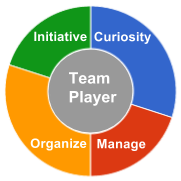
\includegraphics[scale=0.62]{img/personal.png}
%    ~
  \section{Hobbies}
      \href{http://olhares.com/diraol}{\langif{br}{Fotografia}{Photograpy}}
      Tae-Kwon-Do
\end{aside}

\sectionlang{br}{Educação}
\sectionlang{en}{Education}
\begin{entrylist}
  \entry
    {2005 - 2014}
    {\langif{br}{Graduação em Engenharia Elétrica}{Undergraduate in Electrical Engineering}}
    {Universidade de São Paulo, Brazil}
    {\langif{br}{Ênfase Computação - Concluída em 2014}{Minor in Computer and Digital Systems - Concluded in 2014}%
    %Main subjects: Matematics and Physics, Programming, Operational Research, Telecommunication Systems, Digital and Analogical Electronics.\\
    %\emph{Title of the Thesis: "Development, Management and Migrations of web contents and applications".}\\
    %\emph{Thesis activity carried out during an internship period at Atitlan Engineering SRL.}\\
    }
  \entry
    {2000 - 2002}
    {\langif{br}{Ensino Médio}{High School}}
    {Colégio Rio Branco, São Paulo, Brasil}
    {%Scientific Secondary School.\\
    %Main subjects: Matematics, Physics, Computer Science.
    }
\end{entrylist}

\sectionlang{br}{Cursos e Certificações}
\sectionlang{en}{Courses and Certifications}
\begin{entrylist}
  \entry
    {11/2015}
    {Data Science Speacialization}
    {\langif{br}{Universidade Johns Hopkins no Coursera}{Johns Hopkins University on Coursera}}
    {\emph{\langif{br}{Análise Exploratória de Dados}{Exploratory Data Analysis}}\\
    {\langif{br}{Certificado Verificado: }{Verified Certificate: }\scriptsize{\href{https://coursera.org/verify/BCSV3DF2F4}{https://coursera.org/verify/BCSV3DF2F4}}}\\}
  \entry
    {08/2015}
    {Data Science Speacialization}
    {\langif{br}{Universidade Johns Hopkins no Coursera}{Johns Hopkins University on Coursera}}
    {\emph{\langif{br}{Obtenção e Limpeza de Dados}{Getting and Cleaning Data}}\\
    {\langif{br}{Certificado Verificado: }{Verified Certificate: }\scriptsize{\href{https://coursera.org/verify/YFY5YWF3MM}{https://coursera.org/verify/YFY5YWF3MM}}}\\}
  \entry
    {07/2015}
    {Data Science Speacialization}
    {\langif{br}{Universidade Johns Hopkins no Coursera}{Johns Hopkins University on Coursera}}
    {\emph{\langif{br}{Linguagem R}{R Programming}}\\
    {\langif{br}{Certificado Verificado: }{Verified Certificate: }\scriptsize{\href{https://coursera.org/verify/M2NP642ZUE}{https://coursera.org/verify/M2NP642ZUE}}}\\}
  \entry
    {07/2015}
    {Data Science Speacialization}
    {\langif{br}{Universidade Johns Hopkins no Coursera}{Johns Hopkins University on Coursera}}
    {\emph{\langif{br}{As Ferramentas do Cientista de Dados}{Data Scientist’s Toolbox}}\\
    {\langif{br}{Certificado Verificado: }{Verified Certificate: }\scriptsize{\href{https://coursera.org/verify/ELJEYB2D8A}{https://coursera.org/verify/ELJEYB2D8A}}}\\}
  \entry
    {12/2014}
    {\langif{br}{Objetos Pythonicos}{Pythonic Objects}}
    {\langif{br}{PythonPro}{PythonPro}}
    {\href{https://adm.python.pro.br/cursos}{https://adm.python.pro.br/cursos}}
\end{entrylist}

\sectionlang{br}{Publicações}
\sectionlang{en}{Publications}
{\href{http://polignu.org/artigo/twitter-api-elasticsearch-e-kibana-analisando-rede-social}{\textbf{Twitter API, ElasticSearch e Kibana - Analisando a rede social}}\\
\emph{\langif{br}{Tutorial sobre como coletar, processar e analisar dados do Twitter}{Tutorial on how to gather, process and analyse twitter traffic}}\\}\\
{\href{http://diraol.polignu.org}{\textbf{DiRaOLinux}}\\
\emph{\langif{br}{Blog para documentar e compartilhar experiências diárias com software livre}{Blog to document and share daily discovers and issues fixes}}\\}\\
\href{http://polignu.org/administrativo/caderno-polignu-volume-1-software-e-culturas-livres}{\textbf{Caderno do PoliGNU - Vol 1 - Software e Cultura Livres}}\\
\emph{\langif{br}{Material introdutório sobre Software Livre e Cultura Livre}{Introductory material about Free Software and Free Culture (pt-br)}}\\

\sectionlang{br}{Projetos}
\sectionlang{en}{Projects}
%\section{Projects}
\textbf{\langif{br}{Radar Parlamentar}{The Parliamentary Radar}} - \href{http://radarparlamentar.polignu.org/}{http://radarparlamentar.polignu.org/}\\
\langif{br}%
{O Radar Parlamentar é um aplicativo que determina ``semelhanças'' entre partidos \nohyphens{políticos} baseado na análise matemática dos dados de votações de projetos de lei na casa \nohyphens{legislativa}. Existem ainda algumas análises relativas a questões de gênero no Parlamento.\\
Este projeto recebeu 4 premiações desde 2012.}%
{It's a web application that determinates "similarities" between political parties based on the analysis of voting data of legislative houses. There are also some gender analysis from the Parliament. 
This project has been received 4 awards since 2012.}\\
\langif{br}%
{Tecnologias}{Technologies}: Django/Python, R, SQLite/MySQL/Postgres, nginx, uWSGI, D3.js

\textbf{Transparência Hacker \lang{en}{(\textit{Hacker Transparency})}}\\
\langif{br}%
{Membro da comunidade brasileira Transparência Hacker, que atua nas áreas de Governo Aberto, Transparência Pública, Dados Abertos e afins. A comunidade já criou o Ônibus Hacker, participou da criação do \href{http://blog.openingparliament.org/post/72099651071/a-permanent-hacker-space-in-the-brazilian-congress}{\textbf{Laboratório Hacker do Congresso Nacional}}, influenciou na formulação da Lei de Acesso à Informação e do Marco Civil da Internet, dentre outros.}%
{Member of Brazilian Hacker Transparency community, that advocates for OpenGov, Public Transparency, OpenData, etc. The community created the HackerBus, participated on the creation of a \href{http://blog.openingparliament.org/post/72099651071/a-permanent-hacker-space-in-the-brazilian-congress}{\textbf{HackerLab at the Congress}}, influenced the Brazilian Public Information Access act and the ``Marco Civil da Internet'', besides other projects.}

\newpage
\pagenumbering{gobble}% Remove page numbers (and reset to 1)
\begin{aside}
~
~
~
  \section{\langif{br}{Outras Tecnologias}{Other Techs}}
    CartoDB
    Django
    Drupal
    Gimp
  	Git
    Inkscape
    Mediawiki
    MySQL/MariaDB
    NFS
    Nginx
    OpenLDAP
    Postgres
    QuantumGis
    Varnish
    Wordpress
    Xen
\end{aside}

\sectionlang{br}{Eventos}
\sectionlang{en}{Events}
{\footnotesize{Out/15}}  - \href{http://www.hackagenda.com.br/evento/sesi-cultura-digital-2015-hackathon-o-museu-do-seculo-xxi/}{\textbf{SESI Cultura Digital 2015 + Hackathon “O museu do século XXI”}}\\
\langif{br}{Instrutor do workshop ``mapeamento com CartoDB'' e mentor dos grupos participantes do Hackathon}{Instructor of the ``Mapping with CartoDB'' workshop and mentor of the Hackathon participant groups}.

%TODO
{\footnotesize{Ago/15}}  - \href{******}{\textbf{\langif{br}{Seminário de Jornalismo da Faculdade Casper Líbero}{Journalism Seminar on the Casper Líbero University}}}\\
\langif{br}{Debatedor na mesa ******}{Debater on the Discussion about *****}.

{\footnotesize{Jul/13}}  - \href{http://abraji.org.br/congresso/}{\textbf{\langif{br}{9$^o$ Congresso Internacional de Jornalismo Investigativo}{9$^{th}$ Internation Investigative Journalism Congress}}}\\
\langif{br}{Instrutor do workshop ``Programação para Jornalistas''}{Instructor of the ``Coding for journalists'' workshop}.

{\footnotesize{Nov/13}}  - \href{https://knightcenter.utexas.edu/pt-br/blog/00-14390-inscricoes-abertas-para-primeiro-curso-da-anj-com-o-centro-knight-introducao-ao-jornal}{\textbf{\langif{br}{Curso de Introdução ao Jornalismo de Dados}{Introduction to Data Journalism MOOC}}}\\
\langif{br}{Instrutor do módulo ``Programação''. Curso organizado pelo Knight Center e pela \nohyphens{Associação} Brasileira de Jornais}{Instructor of the ``Programming'' module. Course organized by Knight Center and the brazilian National Journals Association}

{\footnotesize{Nov/13}} - \href{http://2.encontro.dados.gov.br/encontro.html}{\textbf{\langif{br}{II Encontro Nacional de Dados Abertos}{II Brazilian National Conference of OpenData}}}\\
\langif{br}{\textit{Chairman} da Trilha de Visualização de Dados}{Chairman of the dataviz trail}

{\footnotesize{Jul/13}} - \href{http://rodadahacker.com/}{\textbf{II RodAda Hacker}}\\
\langif{br}%
{Mentor na segunda edição da ``RodAda Hacker, um workshop de um dia que objetiva dar a mulheres mais autonomia com tecnologias}%
{Mentor on the second edition of ``RodAda Hacker'', a one day workshop that aims to give woman autonomy with techonologies}

{\footnotesize{\langif{br}{Mai/13}{May/13}}} - \href{http://www2013.org/}{\textbf{www2013 Conference}}\\
\langif{br}{Palestrante na mesa ``\textit{eGov and Open Data Camp}'', falando sobre ``\textit{The challenges and opportunities of data journalism}''}%
{Speaker on the ``eGov and Open Data Camp'' discussion, talking about ``The challenges and opportunities of data journalism''}

{\footnotesize{Mar/13}} - \href{http://rodadahacker.com/}{\textbf{I RodAda Hacker}}\\
\langif{br}%
{Mentor na primeira edição da ``RodAda Hacker, um workshop de um dia que objetiva dar a mulheres mais autonomia com tecnologias}%
{Mentor on the first edition of ``RodAda Hacker'', a one day workshop that aims to give woman autonomy with techonologies}

{\footnotesize{\langif{br}{Out/12}{Oct/12}}} - \href{http://yapcbrasil.org.br/2012/talk/110}{\textbf{YAPC::Brasil 2012}}\\
\langif{br}%
{Palestrante: ``Radar Parlamentar: Desvendando a política legislativa''}%
{Speaker: ``The Parliamentary Radar: Unraveling the legislative politics''}

{\footnotesize{Jul/12}} - \href{http://softwarelivre.org/fisl13}{\textbf{\langif{br}{13$^o$ Fórum Internacional de Software Livre (FISL)}{13$^{th}$ Internation Free Software Forum}}}\\
\langif{br}{Apresentação do Projeto Radar Parlamentar no Workshop de Software Livre (WSL)}{Presented the Parliamentary Radar project on the Free Software Workshop (WSL)}

{\footnotesize{\langif{br}{Mai/10}{May/10}}} - \href{http://artigo19.org/infoedireitoseu/?p=560}{\textbf{\langif{br}{O direito ao Acesso à Informação}{The Right to Information Access}}}\\
\langif{br}%
{Palestrante sobre o Direito ao Acesso à Informação num debate na PUC-SP}%
{Speaker on the ``Right to Information Access'' debate at PUC Univeristy}
%
%\\
%
%\begin{flushleft}
%\emph{November 22th, 2014}
%\end{flushleft}
%\begin{flushright}
%
%\end{flushright}
%
%%% This piece of code has been commented by Karol Kozioł due to biblatex errors. 
% 
%\printbibsection{article}{article in peer-reviewed journal}
%\begin{refsection}
%  \nocite{*}
%  \printbibliography[sorting=chronological, type=inproceedings, title={international peer-reviewed conferences/proceedings}, notkeyword={france}, heading=subbibliography]
%\end{refsection}
%\begin{refsection}
%  \nocite{*}
%  \printbibliography[sorting=chronological, type=inproceedings, title={local peer-reviewed conferences/proceedings}, keyword={france}, heading=subbibliography]
%\end{refsection}
%\printbibsection{misc}{other publications}
%\printbibsection{report}{research reports}

\end{document}
